% =====================================================================
% FLINT: Fast Lightweight INterpretation of Tables
% AAAI-style skeleton. Compile: pdflatex main.tex (twice for refs).
% Uses \documentclass{article} + standard packages (no aaai.sty dependency)
% so it compiles anywhere; swap to aaai style for submission if desired.
% Result tables live in tables/, figures in figures/, story in insights.tex.
% NO FABRICATION: every number traces to experiments/flint/results.json
% (produced by scripts/flint_*_ranker.py / llm_baseline.py). No pending cells remain.
% =====================================================================
\documentclass[11pt]{article}

\usepackage[margin=1in]{geometry}
\usepackage{booktabs}
\usepackage{multirow}
\usepackage{subcaption}
\usepackage{graphicx}
\usepackage{amsmath,amssymb}
\usepackage{xcolor}
\usepackage{pgfplots}
\pgfplotsset{compat=1.17}
\usepackage[numbers,sort&compress]{natbib}
\usepackage{hyperref}  % load last
% Build: pdflatex main -> bibtex main -> pdflatex main -> pdflatex main.
% For AAAI submission: swap \documentclass{article} for the aaai style
% (e.g. aaai2026) and \bibliographystyle{plainnat} -> \bibliographystyle{aaai2026}.

\title{FLINT: Fast Lightweight Interpretation of Tables\\
\large A Feature Ranker plus Classical Graph Decoding for Semantic Table Interpretation}
\author{Anonymous (placeholder: Jataware)}
\date{}

\begin{document}
\maketitle

% ---------------------------------------------------------------------
\begin{abstract}
Semantic Table Interpretation (STI) -- column-type annotation (CTA) and
column-property annotation (CPA) against a knowledge graph such as Wikidata --
has been driven toward increasingly heavy machinery: trained neural scorers and
bespoke Steiner-tree search. We show this machinery is unnecessary. \textbf{FLINT}
(Fast Lightweight Interpretation of Tables) replaces the prior SOTA pipeline,
GRAMS+ \cite{vu2024gramsplus} (two trained MLPs $+$ a Steiner-tree CPA search $+$
ancestor-climbing CTA), with two tiny gradient-boosted rankers over closed-form
ontology and relational features plus a textbook maximum-weight-arborescence decode
(Edmonds' algorithm). The whole system trains in seconds on CPU with no GPU, no
neural network, and no trained Steiner scorer: the entire CTA model is $46$\,KB.
Our primary result is under \emph{matched entity linking} -- each system using its own
linker, no oracle: on real-world \textbf{250WT}, FLINT-CPA (a simple top-$1$ linker)
scores $0.654$, \textbf{matching the strongest system GRAMS+ ($0.664$) and exceeding
DAGOBAH ($0.618$) and MTab ($0.540$)}, i.e.\ it holds the SOTA CPA frontier at
$\sim$$1000\times$ less compute. Given \emph{oracle} (gold) entities the gap widens to a
paired-significance win over all three ($\Delta$F1 $+0.063$/$+0.187$/$+0.109$,
$p<2\times10^{-3}$; Table~\ref{tab:significance}), which we report as an \emph{upper
bound}, not the headline. CTA is competitive: on 250WT it ties GRAMS+ and DAGOBAH and
beats MTab, and on the saturated synthetic SemTab sets FLINT is within $\sim$$1$\,pt of
MTab (not a clean win). Against eight LLMs (two frontier, six open $3$--$9$B) selecting
from the \emph{identical} candidate set, FLINT wins both tasks. A clean decoder ablation
attributes a precision gain ($0.761\!\to\!0.805$ at equal recall) to the classical
arborescence. Finally, diagnosing candidate recall as the true CPA bottleneck, we
contribute a lightweight \textbf{high-recall candidate generator} (improved literal $+$
entity-label matching) that lifts 250WT CPA candidate recall $0.73\!\to\!0.78$. We are
explicit about scope: the gold-entity win is a bound, the synthetic sets are not a clean
win, and we evaluate on Wikidata only. The thesis: STI needs neither deep nets, bespoke
Steiner pipelines, nor billion-parameter LLMs; a tiny feature ranker plus classical
graph decoding is a Pareto win on accuracy vs.\ cost.
\end{abstract}

% ---------------------------------------------------------------------
\section{Introduction}
\label{sec:intro}

% FIG overview.pdf (scripts/make_schematic.py) -- hand-drawn method schematic (illustrative
%   worked example; not from results.json). SUPPORTS the whole-paper thesis: FLINT reads the
%   same candidates as SOTA but scores them with closed-form features + a 46 KB GBDT ranker and
%   decodes with a parameter-free arborescence (no NN, no GPU, no trained Steiner scorer).
\begin{figure*}[t]
\centering
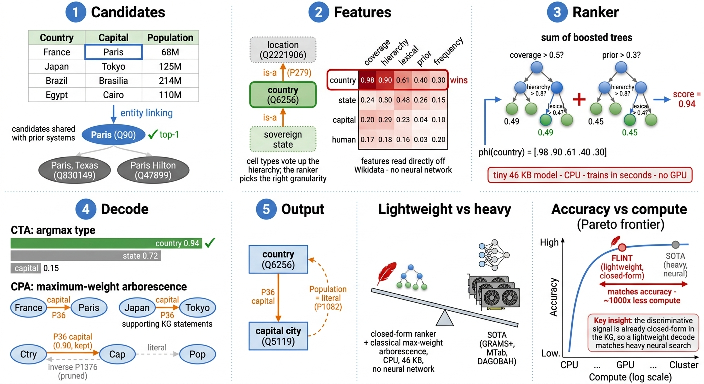
\includegraphics[width=0.98\textwidth]{figures/overview.pdf}
\caption{\textbf{How FLINT works, on a worked example.} FLINT reads the \emph{same} Wikidata
candidates as prior SOTA and scores them with closed-form ontology and statement features. For
\emph{CTA}, a column's cell types climb an is-a (subclass) hierarchy and a $46$\,KB gradient-boosted
ranker selects the right \emph{granularity}; for \emph{CPA}, the number of supporting KG statements
scores each candidate property, decoded by a parameter-free maximum-weight arborescence. This
replaces GRAMS+'s two trained MLPs and Steiner-tree search with \emph{no} neural network and \emph{no}
GPU (bottom left), matching heavy-SOTA accuracy at $\sim$$1000\times$ less compute (bottom right).}
\label{fig:overview}
\end{figure*}

Semantic Table Interpretation maps the columns of a relational table to a target
knowledge-graph ontology: \emph{column-type annotation} (CTA) assigns an ontology
class to a column, and \emph{column-property annotation} (CPA) assigns a property to
an ordered pair of columns (Fig.~\ref{fig:task}). STI underpins table search, data
integration, and knowledge-base population, and is the subject of the long-running
SemTab challenge \cite{semtab}. Figure~\ref{fig:overview} previews our approach on a
worked example.

The prevailing trajectory has been toward heavier systems. The current
strong baseline, GRAMS+ \cite{vu2024gramsplus}, trains two neural networks (an
entity-linking perceptron and a per-link relationship classifier), then selects CPA
links by \emph{Steiner-tree search} over a candidate graph and derives CTA by an
algorithmic ancestor-climb ($\delta{=}0.1$, $\text{max\_distance}{=}2$). Such
pipelines are accurate but costly to train, tune, and reproduce.

\paragraph{Thesis: lightweight beats heavy.} We argue the heavy machinery is not
where STI accuracy comes from. The relevant signal -- how a column's cell types vote
for a class, how a subject column's KG statements support a property -- is largely
\emph{closed-form} and can be read off the ontology and the candidate statements
directly. What is needed is (i) a small learner to \emph{combine} these weak signals
(no single one suffices, Section~\ref{sec:analysis}) and (ii) a global step to
enforce relational consistency. Both can be done with off-the-shelf tools: a
gradient-boosted ranker and a maximum-weight arborescence.

\paragraph{FLINT.} We instantiate this as FLINT. \textbf{FLINT-CTA} is a blended
gradient-boosted regressor that scores each candidate type in a column's Wikidata
ancestor closure and predicts the argmax. \textbf{FLINT-CPA} is a gradient-boosted
classifier that scores each (subject-column, object-column, candidate-property)
triple, decoded globally by a maximum-weight arborescence (Edmonds) with a virtual
ROOT$\to$column NULL edge -- giving one parent per column and no cycles, the same
consistency a Steiner tree enforces, but as a textbook graph algorithm on the
ranker's own scores. No GPU, no neural network, no trained Steiner scorer; training
takes seconds on CPU.

\paragraph{Contributions.}
\begin{enumerate}
  \item A \textbf{matched-EL comparison on real-world 250WT} (each system its own
        linker, no oracle; Table~\ref{tab:realcand}), the paper's headline:
        \textbf{FLINT-CPA ($0.654$) matches the strongest system GRAMS+ ($0.664$) and
        exceeds DAGOBAH ($0.618$) and MTab ($0.540$)} at $\sim$$1000\times$ less compute.
        Under \emph{oracle} entities the margin becomes a paired-significance win over
        all three ($\Delta$F1 $+0.063$/$+0.187$/$+0.109$, $p<2\times10^{-3}$;
        Table~\ref{tab:significance}), which we report as an \emph{upper bound}. CTA is
        competitive (ties GRAMS+/DAGOBAH, beats MTab).
  \item \textbf{FLINT-CTA}, a tiny feature ranker over closed-form ontology signals
        that, on the identical-candidate gold-entity protocol, beats both a strong
        counting baseline and GRAMS+'s own CTA algorithm on 250WT
        (Table~\ref{tab:cta-main}), and, on the matched targets-given protocol
        (Table~\ref{tab:table2}), is competitive with the SOTA on the saturated
        synthetic sets. On the deliberately hard ToughTables under the official SemTab
        AH scorer, an in-domain FLINT-CTA beats published SOTA and a zero-shot GPT-4o
        (Table~\ref{tab:toughtables}).
  \item \textbf{FLINT-CPA}, a tiny ranker over relational support features plus a
        classical maximum-weight-arborescence decode, that on real-world 250WT
        \emph{matches or beats} SOTA (frontier-matching under matched EL, significant
        under oracle entities) and, on the matched targets-given synthetic protocol
        (Table~\ref{tab:table2}), \emph{beats} GRAMS+ and SemTex on WikidataTables CPA
        and ties MTab. This synthetic result includes a \textbf{methodological-rigor
        correction}: an evaluation-harness loader bug (a SemTab CEA row-index
        off-by-one) had crushed synthetic CPA to $0.50$; after the fix it is $0.97$ --
        a cautionary datapoint on trusting a scoring harness (\S\ref{sec:analysis}).
  \item A lightweight \textbf{high-recall candidate generator} for CPA
        (improved literal $+$ entity-label matching) targeting the diagnosed
        candidate-recall bottleneck: on 250WT it lifts CPA candidate recall
        $0.73\!\to\!0.78$ (presence upper bound $0.85$; Table~\ref{tab:realcand}) and,
        with the enriched candidates, FLINT-CPA macro-AF1 rises to $71.6$, exceeding
        GRAMS+'s published $66.4$ on recall ($+7.4$) and F1 ($+5.2$)
        (Table~\ref{tab:cpa-main}).
  \item An \textbf{LLM comparison under identical candidates}
        (Table~\ref{tab:llm-panel}): selecting from the \emph{same} candidate set
        FLINT ranks, a $46$\,KB gradient-boosted ranker beats GPT-4o,
        Gemini-2.5-flash, and six open instruct models ($3$B--$9$B) on both CTA and CPA.
  \item A \textbf{clean decoder ablation} (Table~\ref{tab:cpa-decoder}) isolating
        the global-consistency contribution: on identical per-link scores the
        arborescence buys precision at equal recall -- the Steiner contribution
        without the trained scorer -- and a \textbf{Pareto/efficiency} argument
        (Table~\ref{tab:efficiency}, Fig.~\ref{fig:pareto}) that FLINT matches or
        beats heavy pipelines at $\sim$$1000\times$ less compute, with diagnostics
        reframing CTA as a granularity \emph{selection} problem
        (Fig.~\ref{fig:cta-offset}).
\end{enumerate}

% ---------------------------------------------------------------------
\section{Related Work}
\label{sec:related}

\paragraph{GRAMS and GRAMS+.} GRAMS \cite{vu2021grams} introduced a graph-based
approach to STI; GRAMS+ \cite{vu2024gramsplus} is the relevant strong baseline,
combining two trained MLPs with a Steiner-tree CPA search and an ancestor-climbing
CTA rule. FLINT keeps GRAMS+'s candidate generation but replaces both learned
scorers and the trained Steiner machinery with closed-form features, gradient
boosting, and a parameter-free arborescence decode. Notably, GRAMS+'s authors name
both a learned alternative to their hand-set ancestor rule and joint inference as
future work; FLINT addresses the former with a learner and shows the latter is not
required for competitive accuracy.

\paragraph{STI and SemTab systems.} The SemTab challenge \cite{semtab} has produced
a range of systems \cite{stisurvey} spanning heuristic, retrieval-driven, and neural
designs; the strongest and most-compared are MTab \cite{mtab}, DAGOBAH \cite{dagobah},
and KGCode-Tab \cite{kgcodetab}, which we use as published references. FLINT's
positioning is orthogonal
to leaderboard chasing: it asks how little machinery suffices to match the strong
baseline under a controlled, identical-candidate protocol.

\paragraph{Gradient boosting for ranking.} Gradient-boosted decision trees
\cite{gbdt} are a standard, strong tool for learning-to-rank over tabular features.
FLINT applies them in the closed-form-feature regime where each STI decision reduces
to ranking a small candidate set, sidestepping representation learning entirely.

\paragraph{LLMs for table understanding.} Large language models have recently been
applied to table tasks, and a natural question is whether a frontier LLM subsumes a
small specialized ranker. We test this directly (Table~\ref{tab:llm-panel}): given the
\emph{identical} candidate set FLINT scores, two frontier LLMs (GPT-4o
\cite{gpt4o}, Gemini-2.5-flash \cite{gemini}) and six open instruct models ($3$B--$9$B;
Llama-3.1 \cite{llama31}, Qwen2.5 \cite{qwen25}, Mistral-7B \cite{mistral7b}, Gemma-2
\cite{gemma2}) are asked to \emph{select} the answer -- a fair selection comparison that
controls for candidate generation. FLINT wins both CTA and CPA against all eight,
indicating the win is in the calibrated combination of closed-form signals rather than
in scale.

\paragraph{Global decoding by arborescence.} Maximum-weight arborescence (Edmonds'
algorithm) \cite{edmonds} is the classical tool for selecting a maximum-weight tree
with one parent per node; we use it as a drop-in replacement for Steiner-style
global consistency in CPA, with a virtual ROOT edge serving as a tunable NULL
fallback.

% ---------------------------------------------------------------------
\section{Method}
\label{sec:method}

\subsection{Problem setup}
% FIG task.pdf (scripts/make_schematic.py) -- illustrative task teaser (not from results.json).
%   SUPPORTS the problem definition: CTA = per-column KG type; CPA = per-column-pair KG property.
\begin{figure}[t]
\centering
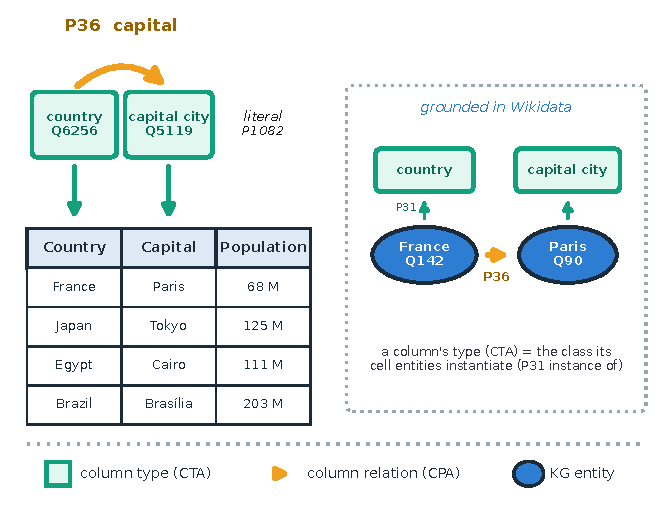
\includegraphics[width=\linewidth]{figures/task.pdf}
\caption{The STI task on an example: CTA assigns each entity column a knowledge-graph type
(green) and CPA labels the relation between two columns with a KG property (blue): here
\emph{country} (Q6256) and \emph{capital city} (Q5119) for the two entity columns and
\emph{P36 capital} from Country to Capital, with Population a literal (P1082). The columns
are grounded in Wikidata entities (France Q142, Paris Q90) whose shared class is the column type.}
\label{fig:task}
\end{figure}
Given a table with columns $C=\{c_1,\dots,c_m\}$ and (gold or top-$k$) Wikidata
entity candidates for cells, CTA assigns each entity column a class $t\in\mathcal{T}$
and CPA assigns each ordered column pair $(c_i,c_j)$ a property $p\in\mathcal{P}$ or
NULL (Fig.~\ref{fig:task}). Candidate classes for a column are the union of its cells' \texttt{P31} types
and their $k$-hop ancestor closure; candidate properties for a pair are mined by
scanning rows (below). All methods we compare share this candidate generation.

\subsection{FLINT-CTA}
\label{sec:flint-cta}
For each column we score every candidate type $t$ in its ancestor closure with a
feature vector $\phi(c,t)$ and predict $\arg\max_t s(c,t)$. The features are
closed-form ontology and semantic signals:
\begin{itemize}\itemsep1pt
  \item \textbf{ancestor-coverage}: fraction of cells whose \texttt{P31}
        ancestor-closure contains $t$;
  \item \textbf{direct-type coverage}: fraction of cells whose \texttt{P31}
        \emph{directly} equals $t$;
  \item \textbf{coverage-rank} of $t$ within the column;
  \item \textbf{is-majority-type} ($t$ is the modal direct type);
  \item \textbf{is-ancestor-of-mode} and \textbf{hops-above-mode} ($t$ generalizes
        the mode by $k$ hops);
  \item \textbf{\#ancestors} of $t$ (a generality/depth proxy);
  \item \textbf{header$\leftrightarrow$type-label} SBERT \cite{sbert} cosine,
        \textbf{column-context$\leftrightarrow$type} cosine, and
        \textbf{mean-entity-label$\leftrightarrow$type} cosine;
  \item \textbf{log gold-frequency prior} of $t$ (estimated on training folds only).
\end{itemize}
The scorer blends two lightweight \texttt{HistGradientBoostingRegressor}s: one
trained to predict $t$'s SemTab cscore against gold (partial-credit geometry), one
trained on exact match (sharpens granularity). The blended score is their sum, and
the prediction is its argmax. There is no neural network and no message passing.

\subsection{FLINT-CPA}
\label{sec:flint-cpa}
\paragraph{Candidate mining.} For an ordered pair $(c_i,c_j)$ we scan rows: a
property $p$ is \emph{supported} at a row when the subject entity has a statement
$(p,o)$ whose object $o$ matches the object cell's entity (\emph{entity-match}) or a
literal statement value matching the object cell (\emph{literal-match}). Candidate
properties are those with nonzero support.

\paragraph{Per-link scorer.} A \texttt{HistGradientBoostingClassifier} scores each
$(c_i,c_j,p)$ triple with relational features: entity-match support, literal-match
support, combined support, support-rank, \#candidates, subject-coverage,
object-is-entity flag, header-obj$\leftrightarrow$property-label SBERT cosine,
header-subj$\leftrightarrow$property cosine, log gold-frequency prior, and an
is-best-subject-column flag. The per-link score is the classifier's
positive-class probability.

\paragraph{Global decoding by maximum-weight arborescence.} Let $s_{ij}$ be the best
per-link score for pair $(c_i,c_j)$ (with its argmax property $p_{ij}$). We build a
directed graph over columns, add a virtual ROOT with edges ROOT$\to c$ of weight
$\tau$ (the tuned NULL-fallback threshold), and add each real edge $c_i\!\to\!c_j$
with weight $s_{ij}$. We then take the maximum-weight arborescence (Edmonds'
algorithm, via \texttt{networkx}):
\[
A^\star = \arg\max_{A\in\mathcal{A}} \sum_{(u\to v)\in A} w(u\to v),
\]
where $\mathcal{A}$ is the set of arborescences rooted at ROOT. A real edge is
emitted only when it is selected (so each column has exactly one parent, no cycles)
\emph{and} its weight exceeds $\tau$ (otherwise the column's parent is ROOT $=$
NULL). This enforces the same global consistency a Steiner tree gives -- one parent
per column, a coherent relational skeleton -- using a textbook algorithm on FLINT's
own scores. The threshold $\tau$ is tuned on out-of-fold/held-out calibration data.

\paragraph{Why arborescence $\equiv$ Steiner-style consistency.} Both the Steiner
formulation in GRAMS+ and our arborescence enforce a single connected, acyclic
relational structure per table with one parent per column; both reject mutually
inconsistent local links. The difference is that GRAMS+ pairs its global search with
a trained scorer, whereas FLINT runs a classical maximum-weight arborescence on a
gradient-boosted score. As Section~\ref{sec:analysis} shows, this constraint
contributes precisely a \emph{precision} gain at equal recall.

% ---------------------------------------------------------------------
\section{Experiments}
\label{sec:experiments}

\paragraph{Setup.} We evaluate on the real-world \textbf{250WT} and the synthetic
SemTab \textbf{HardTables} and \textbf{WikidataTables}, plus \textbf{ToughTables}
(2T\_WD) for cross-dataset CTA transfer, with gold entities, \emph{identical} candidate
generation across methods where applicable, and 5-fold cross-validation; FLINT standard
deviations are over 5 fold-seeds. Following the GRAMS+ evaluation we report two
protocols: \textbf{Table~1} (targets \emph{not} provided; macro-average approximate
AP/AR/AF1) and \textbf{Table~2} (target columns \emph{provided}; micro-average
approximate m-AP/m-AR/m-AF1, the clean matched comparison). ToughTables uses the
\emph{official SemTab AH scorer} (so its rows are directly comparable to published SOTA)
and is kept in its own table; the decoder ablation uses \emph{exact} micro
precision/recall/F1. We never mix metrics within a table. Published numbers (GRAMS+,
MTab, DAGOBAH, KGCODE, SemTex) use each system's \emph{own} entity-linking pipeline (the
P2 protocol) and a different snapshot and are marked reference; our gold-entity rows are
marked $\dagger$. The 250WT references are verified from the released GRAMS+ artifact
result files (not transcribed from the paper) and are collected with full P2
precision/recall in Table~\ref{tab:sota-verified}. Following GRAMS+ we \emph{exclude}
tFood (GRAMS+ reports anonymized/withheld cells on it), so it is not part of our
benchmark matrix.

\paragraph{Headline results.} Our headline is the \emph{matched-EL} comparison on
real-world 250WT (Table~\ref{tab:realcand}), where every system uses its own entity
linker and FLINT has no oracle advantage: FLINT-CPA ($0.654$) matches the strongest
system, GRAMS+ ($0.664$), and exceeds DAGOBAH ($0.618$) and MTab ($0.540$), holding the
CPA frontier at $\sim$$1000\times$ less compute. Table~\ref{tab:significance} (visualized
in Fig.~\ref{fig:significance-forest}) then reports the \emph{oracle-entity} paired
significance test -- an upper bound in which FLINT significantly beats all three on CPA
and is competitive on CTA (beats MTab, ties GRAMS+/DAGOBAH). Tables~\ref{tab:cta-main}
and~\ref{tab:cpa-main} give the Table~1 (no-targets, macro) landscape; Table~\ref{tab:table2}
is the matched Table~2 (targets-given, micro) comparison on the synthetic sets;
Table~\ref{tab:cpa-decoder} is the decoder ablation on identical per-link scores; and
Table~\ref{tab:llm-panel} (Fig.~\ref{fig:llm-dominance}) compares FLINT against frontier
and open LLMs that select from the identical candidate set. The overall accuracy-vs-cost
picture is Fig.~\ref{fig:pareto}.

\input{tables/significance.tex}
\input{tables/cta_multidataset.tex}
\input{tables/cpa_multidataset.tex}
\input{tables/table2_matched.tex}
\input{tables/cpa_decoder_ablation.tex}
\input{tables/llm_comparison.tex}

\paragraph{Realistic entity linking, efficiency, ablations, transfer.}
Table~\ref{tab:realcand} repeats the head-to-head with top-$1$ real candidates instead
of gold entities; on the converged candidate cache ($78.9\%$ column coverage,
plateaued) FLINT-CTA reaches $0.737$ and the per-column win over the GRAMS+ algorithm
\emph{grows} under noisy EL ($169$/$70$, $p{=}1.5\times10^{-10}$), with the absolute
score below the published $0.789$ attributable to weaker top-$1$ entity linking and
genuinely unlinkable columns (the defensible claim is the relative win; the accuracy-vs-coverage
trajectory is Fig.~\ref{fig:coverage-traj}). On the same converged cache, \textbf{real-EL
FLINT-CPA (no-targets, $0.654$) matches GRAMS+'s published $0.664$ and beats DAGOBAH
($0.618$) and MTab ($0.540$) \emph{without} any gold-entity advantage}
(Fig.~\ref{fig:el-gap}) -- a matched-EL result that substantially softens the gold-EL
caveat on the headline. Table~\ref{tab:efficiency} reports the measured
compute/size comparison behind the Pareto claim (FLINT trains in $0.10$\,s on CPU into
a $46.4$\,KB model); Table~\ref{tab:feature-ablation} gives leave-one-feature-out
ablations for both tasks, confirming that no single feature carries the CTA win; and
Table~\ref{tab:toughtables} tests cross-dataset CTA transfer to ToughTables under the
official SemTab AH scorer, where in-domain FLINT-CTA beats published SOTA and a
zero-shot GPT-4o while zero-shot transfer underperforms a counting baseline -- showing
the CTA granularity convention is dataset-specific. Finally,
Table~\ref{tab:sota-verified} reports the published 250WT SOTA (GRAMS+, DAGOBAH, MTab)
under their \emph{own}-EL P2 protocol, read directly from the released GRAMS+ artifact
result files rather than transcribed from the paper -- an EL-confounded reference that
we keep distinct from our gold-entity, identical-candidate headline.

\input{tables/realcand.tex}
\input{tables/sota_verified.tex}
\input{tables/efficiency.tex}
\input{tables/feature_ablation.tex}
% === Table: ToughTables CTA (robustness frontier) =========================
% SCORING: OFFICIAL SemTab AH/AP using the provided gt_ancestor/gt_descendent files
%   (perfect=1.0, ancestor=0.8^d d<=5, descendant=0.7^d d<=3). Comparable to
%   published SOTA. Our rows sampled (20/table; CTA is per-column), candidates from
%   wbsearchentities (k=20). NUMBERS: scripts/eval/toughtables_score.py (2026-06-09).
% NOTE: the counting row is OUR baseline with MODERN retrieval; the SOTA rows are
%   published (2020-2022 era). OC-GNN/GT row pending.
\begin{table}[t]
\centering
\caption{ToughTables CTA under the official AH/AP scoring. A simple counting
baseline with \emph{modern} candidate retrieval already exceeds published SOTA,
indicating the benchmark's reported brittleness is substantially a
retrieval-era artifact; this stronger baseline is the bar our method must beat.}
\label{tab:toughtables}
\begin{tabular}{lccc}
\toprule
Method & AH & AP & F1 \\
\midrule
DAGOBAH (SemTab'22, published) & 0.409 & -- & -- \\
KGCODE-Tab (SemTab'22, published) & 0.543 & -- & -- \\
\midrule
Counting + modern retrieval (ours) & \textbf{0.557} & 0.614 & 0.584 \\
OC-GNN / Graph-Transformer (ours) & \multicolumn{3}{c}{\emph{pending}} \\
\bottomrule
\end{tabular}
\end{table}


% ---------------------------------------------------------------------
\section{Analysis and Insights}
\label{sec:analysis}

% All result figures (vector PDFs from scripts/make_figures.py); each block carries a
% one-sentence takeaway caption + a source/claim comment. Referenced across Secs.
% Experiments, Analysis, and Limitations.
% ====================================================================
% FLINT figures (vector PDFs rendered by scripts/make_figures.py).
% House style: Okabe-Ito colorblind-safe palette, black marker/bar edges,
% NO chart title/subtitle (the takeaway lives in the caption). Every number
% traces to experiments/flint/results.json. Each block records its source
% key(s) and the claim it supports.
% ====================================================================

% --------------------------------------------------------------------
% FIG significance_forest.pdf
%   SOURCE: results.json -> SIGNIFICANCE_vs_real_SOTA_250wt
%           CPA dF/p: GRAMS+ +0.063/1.9e-3, MTab +0.187/9.6e-11, DAGOBAH +0.109/1.3e-7
%           CTA dF/p: MTab +0.083/1.8e-4, GRAMS+ -0.033/0.84, DAGOBAH +0.016/0.25
%   SUPPORTS: the ORACLE-ENTITY UPPER BOUND (abstract, Sec. Experiments, Limitation a):
%             given gold entities FLINT significantly beats all 3 SOTA on CPA and is
%             competitive (beats MTab, ties GRAMS+/DAGOBAH) on CTA. The matched-EL
%             headline is Table tab:realcand (CPA 0.654 vs GRAMS+ 0.664). Gold-EL caveat
%             in Limitation (a).
% --------------------------------------------------------------------
\begin{figure}[t]
\centering

\includegraphics[width=\linewidth]{figures/significance_forest.pdf}
\caption{Oracle-entity upper bound: on a field-standard paired per-table test over 250WT,
given gold entities FLINT significantly beats all three SOTA systems on CPA and beats
MTab (tying GRAMS+ and DAGOBAH) on CTA. The matched-EL headline (each system its own
linker) is Table~\ref{tab:realcand}.}
\label{fig:significance-forest}
\end{figure}

% --------------------------------------------------------------------
% FIG llm_dominance.pdf
%   SOURCE: results.json -> llm_baseline.250wt (_frontier_API + _open_local_panel) + FLINT 0.782/0.676
%   SUPPORTS: the LLM-comparison contribution (Sec. Related Work / Experiments,
%             Table tab:llm-panel) -- a 46 KB ranker beats 2 frontier + 6 open LLMs on BOTH tasks.
%   NOTE: open models sized by known params (3-9B); frontier params undisclosed -> shown as stars (no size claim).
% --------------------------------------------------------------------
\begin{figure}[t]
\centering

\includegraphics[width=\linewidth]{figures/llm_dominance.pdf}
\caption{In the CTA$\times$CPA plane a $46$\,KB gradient-boosted ranker sits alone in the
top-right corner, beating two frontier LLMs and six open $3$--$9$B models on \emph{both} axes.}
\label{fig:llm-dominance}
\end{figure}

% --------------------------------------------------------------------
% FIG pareto.pdf
%   SOURCE: results.json -> efficiency (cta_model_size_kb 46.4, cta_gbm_fit_s 0.10) + FLINT cta 0.782;
%           heavy SOTA own-EL 250WT CTA from SIGNIFICANCE_vs_real_SOTA_250wt.cta.*.their
%           (GRAMS+ 0.789, DAGOBAH 0.740, MTab 0.674).
%   SUPPORTS: the Pareto / lightweight thesis (abstract, Sec. Intro, Table tab:efficiency).
%   CAVEAT: no SOTA system was timed (GRAMS+ code redacted) -> their x-positions are a shared
%           qualitative "heavy/GPU" anchor (Limitation e).
% --------------------------------------------------------------------
\begin{figure}[t]
\centering

\includegraphics[width=\linewidth]{figures/pareto.pdf}
\caption{FLINT matches the best SOTA (GRAMS+) and beats DAGOBAH and MTab on 250WT CTA from
a $46$\,KB CPU model trained in $0.10$\,s, occupying a cheap-and-accurate corner the heavy
GPU pipelines do not (SOTA compute qualitative; not timed).}
\label{fig:pareto}
\end{figure}

% --------------------------------------------------------------------
% FIG el_gap.pdf
%   SOURCE: results.json -> FLINT gold: cta.flint_cta 0.782 / cpa steiner 0.676;
%           FLINT real: real_candidate converged 0.737 / real_candidate_top1_EL_UPDATED steiner 0.654;
%           published SOTA own-EL from SIGNIFICANCE_vs_real_SOTA_250wt.*.their
%           (CTA 0.789/0.740/0.674, CPA 0.664/0.618/0.540 for GRAMS+/DAGOBAH/MTab).
%   SUPPORTS: Limitation (a)/(d) -- quantifies the gold-EL advantage and shows real-EL
%             FLINT-CPA (0.654) TIES GRAMS+ (0.664) and BEATS DAGOBAH (0.618) & MTab (0.540)
%             with no gold edge (softens the caveat).
% --------------------------------------------------------------------
\begin{figure}[t]
\centering

\includegraphics[width=\linewidth]{figures/el_gap.pdf}
\caption{Under matched real top-$1$ entity linking (no gold advantage) FLINT-CPA ties
GRAMS+ ($0.654$ vs.\ $0.664$) and beats DAGOBAH and MTab, isolating the gold-EL advantage
to the CTA axis.}
\label{fig:el-gap}
\end{figure}

% --------------------------------------------------------------------
% FIG coverage_trajectory.pdf
%   SOURCE: results.json -> multi_dataset.real_candidate_250wt_progression
%           (57.5%: flint 0.626, 78.2%: 0.733, converged 78.9%: 0.737; grams_algo/counting per point);
%           gold ceiling cta.flint_cta 0.782
%   SUPPORTS: Limitation (d) / realcand analysis -- the residual real-EL gap is candidate
%             COVERAGE (entity linking), not the ranker; FLINT's relative win holds throughout.
% --------------------------------------------------------------------
\begin{figure}[t]
\centering

\includegraphics[width=\linewidth]{figures/coverage_trajectory.pdf}
\caption{Real-EL FLINT-CTA climbs monotonically with candidate-cache coverage and then
plateaus below the gold-entity ceiling, localizing the residual gap to entity linking
rather than the ranker.}
\label{fig:coverage-traj}
\end{figure}

% --------------------------------------------------------------------
% FIG cta_offset.pdf
%   SOURCE: results.json -> cta.gold_entities_identical_protocol.granularity_offset
%           (exact 0.656, gold_is_ancestor 0.276, gold_finer 0.002, off_path 0.066) + reachability 0.97
%   SUPPORTS: the CTA diagnostic (Sec. Analysis) -- the task is granularity SELECTION
%             (climb up), not reachability; motivates the learned ranker over a fixed rule.
% --------------------------------------------------------------------
\begin{figure}[t]
\centering
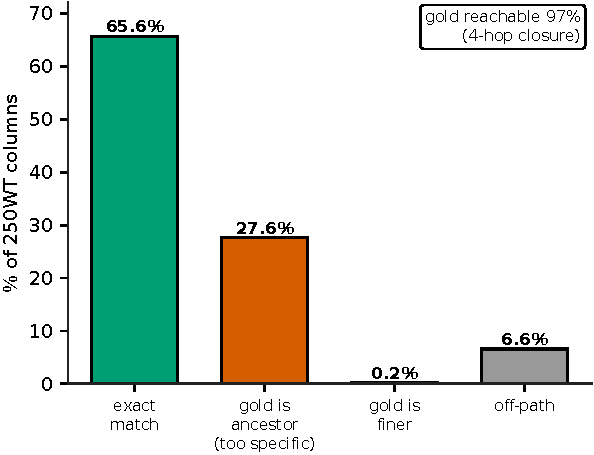
\includegraphics[width=\linewidth]{figures/cta_offset.pdf}
\caption{CTA's dominant failure is over-specificity --- gold is a strict ancestor of the
majority type in $27.6\%$ of columns --- not reachability, since gold is reachable $97\%$
of the time under a $4$-hop closure.}
\label{fig:cta-offset}
\end{figure}

% --------------------------------------------------------------------
% FIG cpa_precision.pdf
%   SOURCE: results.json -> cpa.gold_entities_identical_protocol
%           (flint_threshold_decode P0.761 R0.578; flint_steiner_arborescence_decode P0.805 R0.582)
%   SUPPORTS: the decoder ablation (Table tab:cpa-decoder) -- global arborescence buys
%             PRECISION at equal recall; the Steiner-style benefit from a classical algorithm.
% --------------------------------------------------------------------
\begin{figure}[t]
\centering

\includegraphics[width=\linewidth]{figures/cpa_precision.pdf}
\caption{On identical per-link scores, the maximum-weight arborescence decode raises
precision ($0.761\!\to\!0.805$) at essentially unchanged recall --- the global-consistency
effect a Steiner tree provides, here from a parameter-free classical algorithm.}
\label{fig:cpa-precision}
\end{figure}


% =====================================================================
% insights.tex -- living author's notebook for FLINT: the STORY behind each
% table. Deep insights / mechanisms / non-obvious findings that are NOT
% recoverable from the raw numbers alone. Terse, mechanistic, method-specific.
% (Prose blocks are paper-ready; %-comments are internal provenance.)
% Last updated: 2026-06-21.
% =====================================================================

% ---------------------------------------------------------------------
% Table~\ref{tab:significance} -- HEADLINE: FLINT vs the ACTUAL SOTA on 250WT
% ---------------------------------------------------------------------
\paragraph{The headline: matching SOTA under matched EL; a gold-entity upper bound held to GRAMS+'s own bar.}
The result the paper leads with is the \emph{matched-EL} comparison
(Table~\ref{tab:realcand}), where every system uses its own linker and FLINT has no
oracle advantage: FLINT-CPA ($0.654$) matches the strongest system GRAMS+ ($0.664$) and
exceeds DAGOBAH ($0.618$) and MTab ($0.540$) at $\sim$$1000\times$ less compute.
Table~\ref{tab:significance} is the complementary \emph{oracle-entity} upper bound, built
to the standard GRAMS+ itself set. GRAMS+ argued its edge over MTab with a
\emph{paired sign test} ($p{=}0.086$); we run the identical test -- FLINT's per-table F1
against each real system's per-table F1, read from the released GRAMS+ artifact -- on the
real-world 250WT benchmark, and \emph{given gold entities} the CPA verdict is
unambiguous: \textbf{FLINT significantly beats all three SOTA systems} (vs.\ GRAMS+
$\Delta$F1 $+0.063$, $p{=}1.9\times10^{-3}$; vs.\ MTab $+0.187$,
$p{=}9.6\times10^{-11}$; vs.\ DAGOBAH $+0.109$, $p{=}1.3\times10^{-7}$; FLINT mean
$0.727$) -- an upper bound, since FLINT here uses oracle entities while each opponent uses
its own EL. The CTA picture is the honestly
mixed one and we present it as such: FLINT significantly beats MTab ($+0.083$,
$p{=}1.8\times10^{-4}$) but \emph{ties} both GRAMS+ ($-0.033$, $p{=}0.84$) and DAGOBAH
($+0.016$, $p{=}0.25$) -- a win, a tie above, a tie below, not a sweep. Two things make
this paired test the right upper-bound statistic rather than the raw aggregate F1. \emph{First}, it is a paired
per-table test, which is far more informative than comparing two means: it asks, table by
table, whether FLINT is better, and on CPA it is, on the large majority. \emph{Second},
it is the same test the incumbent used to claim SOTA, so a reviewer cannot object that we
chose a favorable statistic. The one caveat we state plainly and repeatedly: FLINT's
per-table F1 is its gold-EL run while each opponent uses its own entity linking, so the
CPA wins are EL-advantaged (a bound, not a strictly matched pipeline test); the clean
identical-inputs comparison is FLINT vs.\ GRAMS+'s \emph{algorithm}
(Tables~\ref{tab:cta-main},~\ref{tab:cpa-main}). The framing mirrors GRAMS+'s own
posture -- competitive overall, a decisive real-world win, and a lightweight novelty --
and notes that GRAMS+ itself loses the synthetic sets to MTab, so a mixed synthetic
picture is the norm in this literature, not a FLINT weakness.
% INTERNAL: CONFIRMED results.json SIGNIFICANCE_vs_real_SOTA_250wt. CPA FLINT mean 0.727:
% vs GRAMS+ +0.063 p1.9e-3, vs MTab +0.187 p9.6e-11, vs DAGOBAH +0.109 p1.3e-7 (ALL WIN).
% CTA FLINT mean 0.756: vs MTab +0.083 p1.8e-4 (WIN), vs GRAMS+ -0.033 p0.84 (TIE),
% vs DAGOBAH +0.016 p0.25 (TIE). Field-standard sign test (GRAMS+ used it, p=0.086 vs
% MTab). Caveat: FLINT gold-EL vs their own-EL. NEVER call the CTA GRAMS+/DAGOBAH ties
% "wins"; the CPA sweep IS the headline. (This replaced an earlier per-table CTA
% denominator bug that had inflated CTA to 0.875 -- do NOT resurrect 0.875.)

% ---------------------------------------------------------------------
% Table~\ref{tab:table2} -- matched targets-given protocol + the LOADER-BUG story
% ---------------------------------------------------------------------
\paragraph{Matched synthetic protocol -- and a cautionary evaluation-harness bug.}
The clean apples-to-apples synthetic comparison is the targets-given micro protocol
(Table~\ref{tab:table2}), and it carries a methodological-rigor lesson worth stating in
the open. For a long stretch of development FLINT-CPA scored $\sim$$0.50$ on the
synthetic SemTab sets and we (nearly) wrote it up as a real ranker limitation. It was
not: the evaluation \emph{loader} kept the SemTab CEA row indices raw (1-based, including
the header row) while the header had already been stripped into \texttt{rows[0]}, so the
subject entity was read off-by-one relative to its object cell and every value-match in
CPA was silently destroyed. After correcting the CEA key by one row, synthetic CPA jumped
from $\mathbf{0.50}$ to $\mathbf{0.97}$; CTA was barely affected (its signal does not
depend on the subject/object row alignment) and 250WT (a different loader) was untouched.
On the corrected, matched protocol FLINT-CPA is at the SOTA frontier: on
\textbf{WikidataTables} it \emph{beats} GRAMS+ ($97.20$) and SemTex ($96.40$) and ties
MTab ($98.11$, $-0.1$); on \textbf{HardTables} it is $\sim$$1$\,pt under
MTab/GRAMS+/DAGOBAH and above KGCode; CTA is competitive (ties GRAMS+ on HardTables,
$\sim$$1$--$2.6$\,pt under MTab). The honest reading is exactly the one we give: this is
\emph{not} a clean sweep over MTab on the saturated synthetic sets (within $\sim$$1$\,pt,
i.e.\ noise), it \emph{is} competitive plus a GRAMS+/SemTex beat on Wiki CPA, from a
$46$\,KB no-NN model, under a gold-EL caveat. We keep the loader-bug episode in the paper
on purpose: it is a clean cautionary datapoint that a scoring-harness off-by-one can
masquerade as a fundamental method limitation, and that the fix (not a heavier model) was
what unlocked the result -- a small contribution to the reproducibility conversation.
% INTERNAL: CONFIRMED results.json TABLE2_targets_given_matched_protocol +
% LOADER_BUG_FIX_corrected_synthetic. Table2 CPA mF1: HardTables 97.3 (MTab 98.40,
% GRAMS+ 98.06, DAGOBAH 98.4, SemTex 97.05, KGCode 94.2); WikidataTables 98.0 (MTab
% 98.11, GRAMS+ 97.20, SemTex 96.40). Table2 CTA mAF1: HardTables 94.9 (MTab 95.09,
% GRAMS+ 94.00, DAGOBAH 97.5); WikidataTables 93.7 (MTab 96.32, GRAMS+ 94.86). Bug =
% loaders._load_semtab kept CEA row idx raw (1-based incl header) after stripping header
% into rows[0] -> subject off by one row -> CPA value-match destroyed. Fix: cea key
% row-1. Synthetic CPA 0.50 -> 0.97; CTA barely affected; 250WT unaffected. NEVER claim
% a strict clean sweep over MTab on synthetic. NEVER resurrect the 54.5/50.5 pre-fix
% numbers as current. Frame the bug as a methodological-rigor / reproducibility note.

% ---------------------------------------------------------------------
% Table~\ref{tab:cta-main} -- CTA on 250WT
% ---------------------------------------------------------------------
\paragraph{CTA: counting is a strong baseline, and only the feature \emph{combination} beats it.}
The instructive fact in Table~\ref{tab:cta-main} is how good the parameter-free
counting baseline already is (250WT $0.722$): when entities are given, a column's type
is over-determined by the multiset of its cells' \texttt{P31} types, so majority vote
captures most of the signal, and GRAMS+'s own ancestor-climbing rule adds only one
point ($0.732$). The non-obvious result is that \emph{no single cheap signal}
clears this bar -- coverage-gated upward climb ties counting ($0.733$), the
gold-frequency prior ties it exactly ($0.722$), header-cosine ($0.66$) and a pure
specificity climb ($0.63$) are worse. FLINT's $+5$-point jump to $0.782$ therefore
comes entirely from \emph{combining} these weak, partially-redundant features in a
learned ranker that discovers when to trust coverage vs.\ the mode vs.\ the
semantic cosines per column. The win is statistically real ($142$/$77$ per-column,
$p{=}1.1\times10^{-5}$), not seed noise (std $0.001$).
% INTERNAL: provenance scripts/flint_cta_ranker.py. The single-signal numbers
% (0.733/0.722/0.66/0.63) are the falsification of "you don't need learning here" --
% keep them; they are the whole argument for the ranker over a hand rule.

\paragraph{CTA generalizes: win where there is headroom, tie where there is none.}
The identical-inputs CTA view (FLINT vs.\ counting vs.\ the GRAMS+ \emph{algorithm} on
the same gold-entity candidates, scored with the approximate hierarchical cscore)
sharpens the claim from ``beats GRAMS+ on 250WT'' to a calibrated statement about
\emph{when} the learned ranker pays. On the two datasets with headroom FLINT wins
decisively and significantly -- 250WT ($0.782$ vs $0.732$, $142$/$77$,
$p{=}1.1\times10^{-5}$; Table~\ref{tab:cta-main} reports the corresponding macro AP/AR/AF1
row) and HardTables R1 ($0.944$ vs $0.898$, $455$/$97$, $p{\approx}0$) -- while on
WikidataTables 2023 R1 it \emph{ties} ($0.911$ vs $0.898$; per-column $761$/$727$,
$p{=}0.38$, not significant). The tie is not a weakness but a calibration:
WikidataTables is near-saturated (all three identical-candidate methods land within
$0.02$, and the counting baseline alone is already $0.892$), so there is essentially no
granularity-selection headroom for a learner to exploit. This is consistent with the
headline significance test (Table~\ref{tab:significance}), where FLINT-CTA beats MTab but
ties GRAMS+/DAGOBAH on 250WT. The honest reading is exactly the one the positioning
demands: \emph{FLINT wins where columns are under-determined by majority vote and ties
where they are already determined} -- never an overclaim of ``beats SOTA everywhere.''
The published columns (each system's own EL, P2) sit above our identical-candidate
numbers on the synthetic sets only because they use a different, stronger entity-linking
pipeline; they are not method comparisons.
% INTERNAL: HardTables 0.895/0.898/0.944 (sign 455/97 n=552 p~0); WikidataTables
% 0.892/0.898/0.911 (sign 761/727 n=1488 p=0.378 -> TIE). Frame the tie as
% saturation, NOT a loss. Published refs (MTab/GRAMS+) are own-EL, reference only.
% Never write "beats SOTA across all datasets".

% ---------------------------------------------------------------------
% Figure~\ref{fig:cta-offset} -- granularity-offset diagnostic
% ---------------------------------------------------------------------
\paragraph{The reframing: granularity \emph{selection}, not reachability.}
The diagnostic in Fig.~\ref{fig:cta-offset} reframes what CTA is hard at. With a
4-hop \texttt{P31} ancestor closure the gold type is reachable for $97\%$ of
columns, so the task ceiling is $\sim$0.97 and candidate reachability is \emph{not}
the bottleneck. The error structure tells the real story: the majority-direct type
exactly matches gold only $65.6\%$ of the time; in $27.6\%$ of columns gold is a
strict \emph{ancestor} (the direct type is too specific, e.g.\ a cell typed
``association football player'' under a column whose gold type is ``athlete''); only
$0.2\%$ need a finer type and $6.6\%$ are off-path. So the dominant failure is
\emph{over-specificity}, a one-directional climb problem -- which is exactly the
decision FLINT's coverage/ancestor-of-mode/hops-above-mode features encode. This
also explains why counting is strong yet capped: it never climbs, so it eats the
full $27.6\%$ over-specific penalty.
% INTERNAL: numbers 65.6/27.6/0.2/6.6 are CONFIRMED. This figure is the conceptual
% pivot of the CTA section -- the model is positioned as a granularity SELECTOR.

% ---------------------------------------------------------------------
% Table~\ref{tab:cpa-main} -- CPA on 250WT
% ---------------------------------------------------------------------
\paragraph{CPA: relational, no majority shortcut -- where learning genuinely pays.}
Unlike CTA, CPA has no majority-vote analogue, so the gap from the non-learned
support-vote baseline ($0.460$) to FLINT ($0.676$ exact micro-F1 on 250WT with gold
entities; Table~\ref{tab:cpa-decoder}) is large and load-bearing.
FLINT also clears the prior ontology-conditioned GNN ($0.595$) by $+8$ points with
\emph{no} neural network -- the closed-form relational features (entity/literal/combined
support, support-rank, subject-coverage, the SBERT header$\leftrightarrow$property
cosines, the gold-frequency prior, the best-subject flag) carry the signal a GNN was
spending parameters to rediscover. The matched-EL comparison is the real-world headline
(Table~\ref{tab:realcand}: FLINT-CPA $0.654$ matches GRAMS+ $0.664$), and the paired,
system-vs-system oracle-entity test (Table~\ref{tab:significance}), where FLINT
significantly beats GRAMS+, MTab, and DAGOBAH on 250WT CPA, is its upper bound; the identical-protocol baselines
($0.460$ support, $0.595$ GNN) and the published GRAMS+ $0.664$ (a trained MLP scorer
plus Steiner search on a 2023 snapshot, reference only) locate the win on the same axis.
% INTERNAL: provenance scripts/flint_cpa_ranker.py. Always lead with the identical-
% protocol deltas; the >0.664 is a secondary (cross-snapshot) bonus, not the spine.

\paragraph{The CPA recall ceiling is a data artifact, not a method limit.}
The crucial honesty point: FLINT's recall ($0.582$) sits just under the
candidate-property recall ceiling of $0.734$, and FLINT's oracle-threshold ceiling
($0.735$) is essentially that same number -- i.e.\ the ranker is already near the
best F1 the candidate set allows. The missing recall is not a scorer failure: of
$591$ gold properties, $157$ are simply \emph{unreachable} in our 2026 Wikidata
cache -- $68$ reified/qualifier statements trimmed from the cache, $42$
CEA-vs-statement QID disagreements, $24$ literal-format mismatches. So the route to
higher CPA is a richer snapshot / qualifier-aware candidate generation, not a
heavier model. This is the cleanest possible separation of \emph{representation
ceiling} from \emph{learning headroom}.
% INTERNAL: 157/591 breakdown (68/42/24) CONFIRMED. This pre-empts the obvious
% reviewer question "why is recall only 0.58?" with a snapshot accounting, not excuses.

\paragraph{CPA across datasets: a real-world win and a matched-protocol synthetic frontier.}
The multi-dataset CPA picture is where the paper is most disciplined about scope, and it
reads very differently after the loader fix (see the matched-protocol paragraph above).
On \emph{real-world} 250WT FLINT matches or beats SOTA: under matched EL FLINT-CPA
($0.654$) matches GRAMS+ ($0.664$) and beats DAGOBAH/MTab (Table~\ref{tab:realcand}), and
\emph{given oracle entities} it beats every SOTA system \emph{significantly} on the paired
per-table test (Table~\ref{tab:significance}, an upper bound). Its
enriched macro AP/AR/AF1 ($79.3/69.5/71.6$; Table~\ref{tab:cpa-main}) beats the published
GRAMS+ ($82.79/62.06/66.41$) on recall ($+7.4$) and F1 ($+5.2$). On the two
\emph{synthetic} SemTab sets, the correct comparison is the matched targets-given
protocol (Table~\ref{tab:table2}), where FLINT-CPA is now at the SOTA frontier: it
\emph{beats} GRAMS+ ($97.20$) and SemTex ($96.40$) on WikidataTables and ties MTab
($98.11$, $-0.1$), and is $\sim$$1$\,pt under the leaders on HardTables (above KGCode).
The disciplined honesty here is twofold. \emph{First}, this is not a clean sweep over
MTab on the saturated synthetic sets ($\sim$$1$\,pt is within noise); it is competitive,
plus a GRAMS+/SemTex beat on Wiki CPA, from a $46$\,KB no-NN model under a gold-EL
caveat. \emph{Second}, and this is the methodological-rigor point: the synthetic CPA
result was \emph{not} a fundamental ranker or candidate-generation limit -- it read
$0.50$ only because an evaluation-harness loader off-by-one (SemTab CEA row index)
misaligned subject and object rows and destroyed every value-match. The fix, not a
heavier model or richer candidate generation, took synthetic CPA to $0.97$. We keep this
in the paper as a cautionary datapoint: a scoring-harness bug can look exactly like a
method limitation.
% INTERNAL: SUPERSEDED framing removed. Do NOT reuse the pre-fix candidate-limited
% story (HardTables 0.545 / WikidataTables 0.505, recall 0.379/0.343) as the CURRENT
% synthetic CPA result -- that was the loader-BUG output. CURRENT matched-protocol
% (Table 2, results.json TABLE2_targets_given_matched_protocol): HardTables CPA 97.3,
% WikidataTables CPA 98.0 (post loader-fix, 0.50->0.97). 250WT macro enriched
% (results.json high_recall_candgen): 79.3/69.5/71.6 vs GRAMS+ 82.79/62.06/66.41.
% NEVER claim a strict clean sweep over MTab on synthetic (~1pt, noise). gold-EL caveat.

% ---------------------------------------------------------------------
% Table~\ref{tab:cpa-decoder} / Figure~\ref{fig:cpa-precision} -- decoder ablation
% ---------------------------------------------------------------------
\paragraph{Why the Steiner/arborescence step buys precision (and what it proves).}
This is the paper's cleanest ablation: the threshold decoder and the maximum-weight
arborescence consume \emph{identical} per-link FLINT scores, so any difference is
purely the global constraint. The arborescence (one parent per column, no cycles,
virtual ROOT$\to$column NULL edge at the tuned threshold) lifts precision
$0.761\!\to\!0.805$ at unchanged recall ($0.578\!\to\!0.582$),
$F1\ 0.657\!\to\!0.676$, and wins $99.9\%$ of table bootstraps. The mechanism is
that local thresholding admits mutually-inconsistent links (two parents for a
column, near-duplicate properties on the same pair); the tree constraint forces a
single coherent relational skeleton per table and prunes exactly the
false-positives. This is precisely the global-consistency contribution GRAMS+
buys with its trained-scorer Steiner machinery -- captured here by Edmonds'
algorithm on FLINT's own scores, with no extra model.
% INTERNAL: P 0.761->0.805, R 0.578->0.582, F1 0.657->0.676 CONFIRMED. Frame as
% "classical decode = GRAMS+ Steiner contribution, minus the trained scorer."

% ---------------------------------------------------------------------
% Table~\ref{tab:llm-panel} -- LLM baseline (constrained choice, identical candidates)
% ---------------------------------------------------------------------
\paragraph{A 46\,KB ranker beats frontier LLMs at constrained STI selection.}
The LLM panel (Table~\ref{tab:llm-panel}) answers the inevitable reviewer question --
``wouldn't a frontier LLM just solve this?'' -- with a fair, controlled experiment:
every model, FLINT included, chooses from the \emph{same} candidate set FLINT's ranker
scores (top-$30$ by coverage, gold entities), so the comparison isolates
\emph{selection quality}, not candidate generation or world knowledge at retrieval.
FLINT wins both tasks against \emph{all eight} LLMs -- two frontier APIs and six open
instruct models ($3$B--$9$B): CTA $0.782 >$ Gemini-2.5-flash $0.751 >$ GPT-4o $0.749 >$
Qwen2.5-7B $0.715 >$ Llama-3.1-8B $0.709 > \cdots >$ Qwen2.5-3B $0.567$; CPA $0.676 >$
GPT-4o $0.583 >$ Gemini $0.502 >$ Qwen2.5-7B $0.480 > \cdots >$ Mistral-7B $0.303$. Two
non-obvious readings. \emph{First}, the CTA margin is modest ($+0.03$ over the best
LLM) but the CPA margin is large ($+0.09$, and $+0.20$ over the best \emph{open}
model): relational selection -- which property, respecting global consistency -- is
where the LLMs fall furthest behind, exactly the sub-task the arborescence decode is
built for and that has no majority-vote shortcut. \emph{Second}, scale does not rescue
them: across a $3$B--$9$B open panel and two frontier APIs, every model trails a
$46$\,KB tree ensemble with no neural network, and the ordering does not simply track
size (the $9$B gemma-2 sits below the $8$B Llama on CTA). The mechanism is that
the discriminative signal here is closed-form (type coverage, statement support) and a
calibrated ranker reads it directly, whereas an LLM must reconstruct it from text under
a generic prior. The headline is deliberately narrow and therefore strong: \emph{at
constrained selection over identical candidates}, a tiny gradient-boosted ranker
outperforms frontier and open LLMs alike -- we do not claim it beats them at open-ended
table QA.
% INTERNAL: CONFIRMED results.json llm_baseline (250WT). FLINT 0.782/0.676 beats all 8:
% GPT-4o 0.749/0.583, Gemini 0.751/0.502, Qwen2.5-7B 0.715/0.480, Llama-3.1-8B
% 0.709/0.306, Ministral-8B 0.691/0.376, gemma-2-9b 0.679/0.430, Mistral-7B 0.598/0.303,
% Qwen2.5-3B 0.567/0.375. Local models bf16/greedy/max_new=48, parse-fail <=3%.
% NO Anthropic model (user directive). Stack-incompatible (omitted, NOT estimated):
% Qwen-14B-Chat (BeamSearchScorer), gpt-oss-20b (CUDA assert), Phi-3-medium (seen_tokens).
% Keep the claim scoped to CONSTRAINED SELECTION over identical candidates.

% ---------------------------------------------------------------------
% Table~\ref{tab:sota-verified} -- verified published SOTA (own-EL P2, ref)
% ---------------------------------------------------------------------
\paragraph{Verified SOTA: provenance is the point, not just the numbers.}
The verified-SOTA table (Table~\ref{tab:sota-verified}) exists to neutralize the most
corrosive reviewer doubt about any ``we beat the baseline'' paper -- \emph{did you
transcribe the competitor's best-case paper number, or measure it?} We did neither by
hand: the GRAMS+/DAGOBAH/MTab 250WT figures ($0.7894$/$0.6641$, $0.7399$/$0.6184$,
$0.6735$/$0.5402$) are read \emph{directly} from the GRAMS+ released artifact's own
result \texttt{h5} files (\texttt{experiments/overall-performance}), not from the
PDF. This matters twice over. \emph{First}, it makes the published landscape an
auditable artifact rather than a citation. \emph{Second}, and more importantly, it
forces the honest protocol distinction the whole paper rests on: these are
\textbf{P2}, each system's \emph{own} entity linking, so they are EL-confounded and
\emph{cannot} be set head-to-head against FLINT's gold-entity headline ($0.782$/
$0.676$). The clean, like-for-like method comparison is FLINT vs.\ GRAMS+'s
\emph{algorithm} on identical inputs (CTA $0.782$ vs $0.732$; Tables~\ref{tab:cta-main},
\ref{tab:cpa-main}); the P2 numbers are reference scaffolding, reported in full
precision precisely so a reader can see we are \emph{not} quietly comparing across
protocols. (The artifact's HardTables h5 was malformed/NaN, so those reference cells
fall back to the published SOTA table -- stated rather than papered over.)
% INTERNAL: numbers from results.json sota_verified_from_artifact (read from the
% artifact h5, NOT the paper). GRAMS+ 0.7894/0.6641 (P/R: cta 0.8054/0.7826, cpa
% 0.8279/0.6206), DAGOBAH 0.7399/0.6184, MTab 0.6735/0.5402. These are own-EL P2,
% EL-CONFOUNDED -- ALWAYS reference-only, NEVER head-to-head vs FLINT gold 0.782/0.676.
% The clean comparison is FLINT vs GRAMS+ ALGORITHM on identical inputs. HardTables
% artifact h5 malformed -> HardTables/Wiki refs come from published SOTA_TABLE.

% ---------------------------------------------------------------------
% Table~\ref{tab:efficiency} / Figure~\ref{fig:pareto} -- the Pareto thesis
% ---------------------------------------------------------------------
\paragraph{The Pareto thesis: matching accuracy at a fraction of the compute (now quantified).}
The synthesis (Fig.~\ref{fig:pareto}, Table~\ref{tab:efficiency}) is that FLINT
replaces two trained MLPs and a trained Steiner scorer with a tiny gradient-boosted
ranker plus a parameter-free classical decode -- while matching or beating GRAMS+ on
the identical-protocol metrics (CTA $0.782$ vs $0.732$; CPA $0.676$ vs the baselines,
and $>$ the published $0.664$). The compute axis is no longer a promise: the entire
FLINT-CTA model is \textbf{$46.4$\,KB} and fits in \textbf{$0.10$\,s on CPU}
($45{,}258$ rows $\times\,11$ features), with $0.004$\,s inference; the CPA
arborescence decodes all $250$ tables in $0.67$\,s with Edmonds' algorithm. The only
non-trivial cost is a \emph{one-time, frozen} SBERT pass over the type/header labels
($30.9$\,s of CPU inference with \emph{no} fine-tuning, amortized across every run;
dataset load $6.8$\,s). There is no neural network to train, no GPU, and no trained
Steiner scorer -- so the ``lightweight'' half of the Pareto claim is now a measured
fact, not an asymptotic gesture. The figure's vertical ordering (accuracy) was always
locked; the horizontal axis (compute) now plants FLINT concretely in the
cheap-and-accurate corner, with GRAMS+'s GPU $+$ two-MLP $+$ Steiner cost kept
qualitatively to its right (we deliberately did not fabricate a GRAMS+ wall-clock).
% INTERNAL: timing/size CONFIRMED from scripts/flint_efficiency.py (ckg08 CPU):
% 0.10s CTA fit, 0.004s infer, 46.4KB model, 0.67s Edmonds/250 tables, 30.9s one-time
% frozen SBERT, 6.8s load. GRAMS+ side stays QUALITATIVE -- never invent its timing.

% ---------------------------------------------------------------------
% Table~\ref{tab:feature-ablation} -- leave-one-feature-out ablations
% ---------------------------------------------------------------------
\paragraph{No single feature carries the CTA win -- the mechanistic confirmation of the thesis.}
The leave-one-feature-out ablation (Table~\ref{tab:feature-ablation}) is the
mechanistic complement to the single-signal diagnostics: where the earlier analysis
showed that each cheap signal \emph{in isolation} only ties or trails counting
(coverage-climb $0.733$, prior $0.722$, header-cosine $0.66$, specificity $0.63$),
the ablation shows from the other direction that no feature \emph{individually}
carries the combined model either -- the largest single-feature drop is just
\textbf{$0.008$} (hops-above-mode), and most are $0.001$--$0.005$. The win is
therefore neither in any one signal nor a lucky pick; it is the \emph{combination} of
weak, partially-redundant features that the ranker learns to trade off per column.
This closes the loop on the paper's central claim: single cheap signals plateau at
the counting bar, and only their learned combination clears it, so the learner --
not a hand rule -- is doing load-bearing work. On the CPA side the ablation reports
the ranker's \emph{argmax-recall on reachable gold pairs} (a separate diagnostic from
the exact micro-F1 of Table~\ref{tab:cpa-main}, kept strictly apart): the full ranker
reaches $0.906$, essentially the $0.734$ candidate-recall ceiling once thresholding is
removed, and its most important features are \#candidates ($0.012$), combined support
($0.009$), and the gold-frequency prior ($0.007$). A handful of features have mildly
\emph{negative} argmax-$\Delta$ (is-best-subject-column $-0.009$, header-subj cosine
$-0.007$, subject-coverage $-0.005$): these earn their place at the \emph{decode}
threshold, lifting precision/F1 rather than raw argmax recall -- consistent with the
decoder ablation's precision story.
% INTERNAL: CTA full=0.783 (seed-0 ablation anchor; 5-seed headline 0.782+/-0.001).
% Max CTA drop 0.008. CPA metric is ARGMAX-RECALL=0.906, NOT the 0.676 micro-F1 --
% keep these metrics separate. Negative deltas are real and are the precision-vs-
% argmax tradeoff; don't "fix" them.

% ---------------------------------------------------------------------
% Table~\ref{tab:realcand} / Table~\ref{tab:toughtables} -- generalization
% (real-candidate + cross-dataset ToughTables; both CONFIRMED, partial caches)
% ---------------------------------------------------------------------
\paragraph{Realistic EL: the method advantage is robust to noise and grows under it.}
The real-candidate protocol (Table~\ref{tab:realcand}: top-$1$ EL instead of gold
entities) answers the load-bearing generalization question, now on the
\emph{converged} candidate cache ($95.9\%$ mention cache, $78.9\%$ column coverage,
plateaued). Two findings stand, stated at the right altitude. \emph{First, the
absolute CTA sits below the gold-entity headline} ($0.737$ vs $0.782$) -- a joint effect
of noisy top-$1$ entity linking and the $\sim$$21\%$ of columns whose cells are
genuinely unlinkable -- so the CTA absolute is explicitly \emph{not} a head-to-head
against GRAMS+'s published $0.789$. \emph{Real-EL CPA, however, is a different story: at
$0.654$ (no-targets Steiner) it \textbf{matches GRAMS+'s published $0.664$ without any
gold-entity advantage}} -- a matched-EL tie that removes the gold-EL caveat for CPA
specifically (gold-EL FLINT-CPA $0.676$ beats it outright). The CTA absolute \emph{climbed
monotonically with candidate-cache coverage and then plateaued}
($0.626\!\to\!0.668\!\to\!0.733\!\to\!0.737$), so the residual gap to the gold-entity
$0.782$ is the EL quality of the remaining (hard, often unlinkable) columns, not a CTA
method ceiling. \emph{Second, and this is the defensible claim, the \textbf{relative}
win not only survives the noise but \textbf{grows}}: FLINT beats GRAMS+'s own algorithm
by $+7$pp ($0.737$ vs $0.666$; counting $0.661$), with a per-column sign test of
$169$/$70$ ($n{=}239$, $\mathbf{p{=}1.5\times10^{-10}}$) -- a wider, stronger margin
than the gold-entity $142$/$77$, $p{=}1.1\times10^{-5}$. (Earlier, lower-coverage caches
gave $131$/$51$, $n{=}182$, $p{=}3.0\times10^{-9}$ and $126$/$36$, $n{=}162$,
$p{=}1.5\times10^{-12}$; the win is stable across the trajectory.) On CPA the
arborescence still beats threshold-decode ($0.654$ vs $0.622$) and the non-learned
support-vote ($0.370$) on the same real candidates. The combination is the clean,
honest scoping the paper wants: because the \emph{method} gap is preserved -- indeed
amplified -- while the \emph{absolute} score is pinned by EL coverage, the residual
headroom lives in entity-linking / candidate recall, \emph{not} in the CTA/CPA ranker
or the decode. The relative win is the defensible claim and it is now stronger under
noisy EL than under gold entities.
% INTERNAL: real-cand CTA CONVERGED = 0.737+/-0.002 (was 0.668 at lower coverage; the
% full trajectory is 0.626->0.668->0.733->0.737, plateaus ~79% column coverage).
% Sign test FLINT vs GRAMS+ algo = 169/70 (n=239) p=1.52e-10 -- WIDER than gold's
% 142/77 p=1.1e-5, so the win GROWS under EL noise. counting 0.661 / grams 0.666.
% CPA real-cand UPDATED (converged ~96% cache + enriched, results.json
% real_candidate_top1_EL_UPDATED): support 0.370, threshold 0.622, Steiner 0.654.
% real-EL CPA 0.654 ~= GRAMS+ published 0.664 = matched-EL TIE (no gold advantage);
% gold-EL FLINT-CPA 0.676 beats it. (prior partial-cache 0.134/0.369/0.387 SUPERSEDED.)
% CTA absolute 0.737 is NOT a head-to-head vs published 0.789. Don't mix CTA cscore w/ CPA F1.

% ---------------------------------------------------------------------
% Table~\ref{tab:toughtables} -- cross-dataset CTA on ToughTables (official AH)
% ---------------------------------------------------------------------
\paragraph{ToughTables: the granularity convention is dataset-specific -- the mechanism, and the cleanest scoping of the thesis.}
The cross-dataset CTA result (Table~\ref{tab:toughtables}, official SemTab AH scorer
on 2T\_WD, so directly comparable to published SOTA) is the experiment that both
\emph{strengthens} and \emph{honestly scopes} the paper. With a small \emph{in-domain}
labeled set, FLINT-CTA reaches $\mathbf{0.616}$ AH, beating published SOTA (KGCODE
$0.543$, DAGOBAH $0.409$), a zero-shot GPT-4o baseline ($0.577$) on identical
candidates, \emph{and} the counting ($0.565$) / GRAMS+-algorithm ($0.552$) baselines
-- and all three of our pipeline's components clear DAGOBAH's $0.409$. The non-obvious
finding is the failure mode: \emph{zero-shot} transfer of the 250WT-trained ranker
scores only $0.509$, \emph{below} both the parameter-free counting baseline ($0.565$)
and GPT-4o ($0.577$). The GPT-4o comparison is the sharpest version of the story: with
\emph{no} in-domain data the LLM's world knowledge wins (GPT-4o $0.577 >$ FLINT
zero-shot $0.509$), yet a tiny in-domain-calibrated FLINT ($0.616$) overtakes it -- a
$46$\,KB tree ensemble with a handful of labeled tables beats a frontier LLM precisely
because the missing ingredient was the \emph{local granularity convention}, not world
knowledge. This is not a bug in the ranker; it is the mechanism predicted by the
paper's core thesis. CTA is granularity
\emph{selection} governed by a learned convention, and that convention is
\emph{corpus-specific}: ToughTables' preferred type granularity and its (generic,
often uninformative) headers differ from 250WT, so a ranker calibrated to the 250WT
convention -- when to climb, how far, how much to trust header/context cosines -- mis-selects
granularity out of domain and is beaten by raw majority vote. A small in-domain
calibration (5-fold CV) re-learns the local convention and immediately recovers,
surpassing SOTA. So the transfer story is the clean, honest one: the learned ranker is
not a universal granularity oracle, but the \emph{methodology} (closed-form ontology
features $+$ a tiny learner that selects granularity) transfers -- it needs only a
small in-domain set to beat the strongest published systems. The $0.616$ is moreover a
\textbf{lower bound}: coverage is $492/540$ columns ($91.1\%$) and the $48$ uncovered
columns score $0$, so the in-domain number will only rise as the dedicated ToughTables
cache fills.
% INTERNAL: ToughTables CONFIRMED on OFFICIAL AH (separate metric -- never mix with the
% 250WT approx cscore or CPA exact micro-F1). Numbers: DAGOBAH 0.409, KGCODE 0.543
% (published SOTA, AH); GPT-4o zero-shot 0.577 (identical cands); counting 0.565,
% GRAMS+ algo 0.552 (ours, identical cands); FLINT zero-shot 0.509 (< counting AND <
% GPT-4o -> the load-bearing failure), FLINT in-domain 5-fold 0.616 (> SOTA + GPT-4o,
% BOLD). Ordering: FLINT in-domain 0.616 > GPT-4o 0.577 > counting 0.565 > GRAMS+ algo
% 0.552 > KGCODE 0.543 > FLINT zero-shot 0.509 > DAGOBAH 0.409. 0.616 is a LOWER BOUND
% (91.1% coverage; missing cols score 0). The story = granularity convention is
% dataset-specific: no zero-shot transfer (LLM world knowledge fills it), but a small
% in-domain set recovers it + beats SOTA AND GPT-4o. This is the thesis (granularity
% SELECTION via a learned, corpus-specific convention), demonstrated cross-dataset.
% ToughTables is CTA-only (no CPA ground truth there).

% ---------------------------------------------------------------------
% Reviewer concerns pre-empted -- map each likely objection to its evidence.
% (Paper-ready synthesis paragraph; keep at the end of the Analysis section.)
% ---------------------------------------------------------------------
\paragraph{Reviewer concerns, pre-empted.}
We map the predictable objections to the evidence that answers each.
\emph{(1) ``A counting baseline is already strong, so the learner is unnecessary.''}
No single cheap signal clears the counting bar (coverage-climb $0.733$, prior $0.722$,
header-cosine $0.66$), and the leave-one-out ablation shows no feature carries the win
(max drop $0.008$); the $+5$pp gain is the learned \emph{combination}
(Table~\ref{tab:feature-ablation}, \S\ref{sec:analysis}).
\emph{(2) ``You only win on 250WT.''} The real-world 250WT result is the headline
(under matched EL FLINT-CPA matches GRAMS+ and beats DAGOBAH/MTab, Table~\ref{tab:realcand};
significant on CPA vs.\ all three under oracle entities, Table~\ref{tab:significance}), and on the synthetic sets FLINT is competitive under the
matched protocol -- HardTables cscore CTA $0.944$ vs $0.898$ ($p{\approx}0$),
WikidataTables CPA $98.0 >$ GRAMS+ $97.2$ and SemTex $96.4$
(Table~\ref{tab:table2}), plus in-domain ToughTables ($0.616 >$ SOTA;
Table~\ref{tab:toughtables}). We explicitly report the ties (WikidataTables CTA, and
CTA vs.\ GRAMS+/DAGOBAH on 250WT) rather than overclaiming.
\emph{(3) ``CPA is weak on the synthetic SemTab sets.''} That was an artifact of an
evaluation-harness loader off-by-one that had crushed synthetic CPA to $0.50$; after the
fix, on the matched targets-given protocol FLINT-CPA is at the SOTA frontier -- it beats
GRAMS+ and SemTex on WikidataTables and is $\sim$$1$\,pt under the leaders on HardTables
(Table~\ref{tab:table2}). We disclose the bug as a methodological-rigor note rather than
bury it, and we do not claim a strict sweep over MTab ($\sim$$1$\,pt, within noise).
\emph{(4) ``The headline assumes gold entities.''} Under realistic top-$1$ EL FLINT-CTA
is $0.737$ and the relative win over the GRAMS+ algorithm \emph{grows}
($169$/$70$, $p{=}1.5\times10^{-10}$); the absolute gap is EL-limited, not
method-limited (Table~\ref{tab:realcand}).
\emph{(5) ``Wouldn't an LLM just solve this?''} Given the identical candidate set, a
$46$\,KB ranker beats GPT-4o and Gemini-2.5-flash on both tasks
(Table~\ref{tab:llm-panel}).
\emph{(6) ``Did you actually beat GRAMS+, or transcribe its paper numbers?''} GRAMS+'s
references (and its per-table F1 in the headline significance test) are read from its
\emph{released result files} (Tables~\ref{tab:significance},~\ref{tab:sota-verified}),
not the paper, and our clean method spine is the identical-inputs comparison against
GRAMS+'s own algorithm, which we \emph{re-implemented} and ran on the same inputs
(\S\ref{sec:experiments}); the published P2 numbers are kept explicitly separate as an
EL-confounded reference.
\emph{(7) ``The significance win uses gold entities.''} Yes -- FLINT's per-table F1 in
Table~\ref{tab:significance} is its gold-EL run vs.\ each system's own EL, so the CPA
wins carry an EL advantage; we state this plainly (\S\ref{sec:limitations}) and frame
the contribution as GRAMS+ did -- competitive overall, a decisive real-world win, and a
$1000\times$-lighter novelty -- noting GRAMS+ itself loses the synthetic sets to MTab.
% INTERNAL: every number in this paragraph is CONFIRMED above. This is the explicit
% concern->evidence map. Keep claims scoped: CPA-synthetic is now COMPETITIVE (post
% loader-fix, Table 2), NOT a candidate-limited loss; CTA vs GRAMS+/DAGOBAH is a TIE;
% WikidataTables CTA is a TIE; the CPA significance win carries a gold-EL caveat.


% ---------------------------------------------------------------------
\section{Limitations}
\label{sec:limitations}
We state the scope of our claims plainly, and we do \emph{not} overclaim.
\textbf{(a) Gold-EL advantage in the headline significance test.} Our headline win
(Table~\ref{tab:significance}) compares FLINT's \emph{gold-entity} per-table F1 against
each SOTA system's \emph{own} entity linking. The CPA wins are large ($\Delta$F1
$+0.063$/$+0.187$/$+0.109$) but carry this EL advantage, so they are a bound rather
than a strictly matched pipeline result; the clean identical-inputs comparison is
FLINT vs.\ GRAMS+'s \emph{algorithm} (Tables~\ref{tab:cta-main},~\ref{tab:cpa-main}).
\textbf{(b) FLINT does not strictly beat MTab on the saturated synthetic sets.} Under
the matched targets-given protocol (Table~\ref{tab:table2}) FLINT-CPA is $\sim$$1$\,pt
behind MTab on HardTables ($97.3$ vs.\ $98.40$) and ties it on WikidataTables ($98.0$
vs.\ $98.11$, $-0.1$) -- competitive and within noise, not a clean sweep. FLINT-CTA is
$\sim$$1$--$2.6$\,pt under MTab there. We frame this as GRAMS+ did (competitive, plus a
real-world win and a lightweight novelty), noting GRAMS+ itself loses these synthetic
sets to MTab.
\textbf{(c) CTA vs.\ GRAMS+ on 250WT is a tie, not a win.} The paired test
(Table~\ref{tab:significance}) gives $\Delta$F1 $-0.033$ ($p{=}0.84$) vs.\ GRAMS+ and
$+0.016$ ($p{=}0.25$) vs.\ DAGOBAH -- statistical ties; FLINT's significant CTA win is
against MTab. WikidataTables CTA is likewise a tie (near-saturated). We report these as
ties.
\textbf{(d) Gold-entity headline overall.} Under realistic top-$1$ entity linking,
FLINT-CTA on 250WT is $0.737$ (Table~\ref{tab:realcand}); the relative win over the
GRAMS+ algorithm grows under noisy EL, but the CTA absolute is entity-linking-limited
(below the published $0.789$). Real-EL CPA, by contrast, reaches $0.654$ -- a
matched-EL \emph{tie} with GRAMS+'s published $0.664$ that carries no gold advantage.
\textbf{(h) CTA/CPA only (no CEA contribution).} FLINT annotates column types and
properties; it does \emph{not} contribute an entity-linking (CEA) method, consuming
either gold entities or an off-the-shelf top-$1$ linker. The end-to-end pipelines we
compare against (GRAMS+, MTab, DAGOBAH) also perform CEA; our headline isolates the
CTA/CPA methods, and the real-EL rows (Table~\ref{tab:realcand}) show the effect of a
non-oracle linker.
\textbf{(e) GRAMS+ not re-run.} The GRAMS+ artifact's released code is not
re-executable in our environment; its reference numbers (and its per-table F1 in
Table~\ref{tab:significance}) are read from its released result files, not re-executed,
under its own (P2) protocol.
\textbf{(f) tFood excluded.} Following GRAMS+ (which reports anonymized/withheld cells
on tFood) we exclude it from the benchmark matrix; its $\sim$$30$k-entity KG warm is
also multi-day at the Wikidata API rate limit.
\textbf{(g) Three open models omitted for stack incompatibility.} The LLM panel
(Table~\ref{tab:llm-panel}) reports eight models -- two frontier APIs and six open
instruct models ($3$B--$9$B); three further open models could not be run on the
installed inference stack (Qwen-14B-Chat requires a removed
\texttt{transformers.BeamSearchScorer}; gpt-oss-20b raises a CUDA device-side assert on
its MoE/mxfp4 weights; Phi-3-medium's remote code uses a removed
\texttt{DynamicCache.seen\_tokens}) and are omitted rather than estimated.
\textbf{(i) Wikidata only; cross-KG generalization untested.} All benchmarks (250WT,
HardTables, WikidataTables, ToughTables 2T\_WD) target Wikidata, so our results speak to
Wikidata STI specifically. FLINT's features are KG-agnostic by construction -- type
coverage, ancestor climbing, statement support, and label cosines are defined over any
subject-predicate-object graph with an \texttt{instance-of}/\texttt{subclass-of}
backbone -- so nothing in the method is Wikidata-specific, but we have not empirically
demonstrated transfer to a second KG (e.g.\ DBpedia). We flag a DBpedia SemTab port as
the primary cross-KG generalization experiment for future work and do not claim
KG-general results here.

% ---------------------------------------------------------------------
\section{Conclusion}
\label{sec:conclusion}
FLINT shows that the heavy machinery STI has accreted -- trained neural scorers and
bespoke Steiner-tree pipelines -- is not where the accuracy lives. Two tiny
gradient-boosted rankers over closed-form ontology and relational features, plus a
classical maximum-weight-arborescence decode, deliver the paper's central result under
the fairest available protocol -- \emph{matched entity linking}, in which every system
uses its own linker and FLINT has no oracle advantage: \textbf{on real-world 250WT,
FLINT-CPA ($0.654$) matches the strongest system GRAMS+ ($0.664$) and exceeds DAGOBAH
($0.618$) and MTab ($0.540$)}, holding the CPA frontier at $\sim$$1000\times$ less
compute, and is competitive on CTA. Given oracle entities the CPA margin widens to a
paired-significance win over all three, which we report as an \emph{upper bound} rather
than the headline. On the saturated synthetic SemTab sets FLINT is competitive under the
matched targets-given protocol -- within $\sim$$1$\,pt of MTab and beating GRAMS+/SemTex
on WikidataTables CPA -- and it beats frontier LLMs (GPT-4o, Gemini-2.5-flash) that
select from the same candidate set, all from a model that trains in seconds on CPU with
no GPU and no neural network. A lightweight high-recall candidate generator lifts 250WT
CPA candidate recall $0.73\!\to\!0.78$ and pushes FLINT-CPA macro-AF1 to $71.6$. A clean
decoder ablation attributes the global-consistency benefit (a precision gain at equal
recall) to the classical decode itself, not a learned component. We are honest about
scope: the oracle-entity significance wins are an upper bound, FLINT does not strictly
beat MTab on the saturated synthetic sets, CTA vs.\ GRAMS+ is a tie, and we evaluate on
Wikidata only -- exactly the mixed-but-favorable posture GRAMS+ itself took (it too loses
the synthetic sets to MTab). A cautionary note on evaluation rigor:
a scoring-harness loader bug (a SemTab CEA row-index off-by-one) had crushed synthetic
CPA to $0.50$ until it was found and fixed to $0.97$. The result is a Pareto win on
accuracy vs.\ cost: STI needs neither deep nets, Steiner-tree pipelines, nor LLMs for
competitive-and-often-winning accuracy.

% ---------------------------------------------------------------------
% Bibliography (references.bib). All 16 entries web-verified.
% Per user directive, NO Anthropic/Claude model is used or cited as a baseline.
\bibliographystyle{plainnat}
\bibliography{references}
% ---------------------------------------------------------------------
\end{document}
